% Gabarit pandoc des corrigés publiés (brut et guidé). Contenu sans marque ni nom de site.
% Compilation : lualatex (latexmk -lualatex).
% Le Markdown reste la source unique : ne pas éditer ce fichier .tex à la main.
\documentclass[11pt,a4paper]{article}

% --- Moteur, polices (Latin Modern) et langue ---------------------------------
\usepackage{iftex}
\ifLuaTeX\else\errmessage{Ce document se compile avec lualatex}\fi
\usepackage{amsmath,amssymb,mathtools}
\usepackage{fontspec}
% mathrm=sym : \mathrm prend ses glyphes dans la police mathématique (ℓ, μ, Ω), comme KaTeX.
\usepackage[math-style=TeX,bold-style=TeX,mathrm=sym]{unicode-math}
% Repli pour les glyphes absents de Latin Modern (indices et exposants Unicode,
% flèches, filets des schémas en texte, symboles) : DejaVu, puis Latin Modern Math
% (ℓ, lettres mathématiques Unicode des légendes).
\directlua{
  luaotfload.add_fallback("repliTexte", {"DejaVuSerif:mode=harf;", "DejaVuSans:mode=harf;", "file:latinmodern-math.otf:mode=harf;"})
  luaotfload.add_fallback("repliMono", {"DejaVuSansMono:mode=harf;", "DejaVuSans:mode=harf;", "file:latinmodern-math.otf:mode=harf;"})
}
\setmainfont{Latin Modern Roman}[RawFeature={fallback=repliTexte}]
\setsansfont{Latin Modern Sans}[RawFeature={fallback=repliTexte}]
\setmonofont{Latin Modern Mono}[RawFeature={fallback=repliMono}]
\setmathfont{Latin Modern Math}
\usepackage[french]{babel}
\frenchsetup{SmallCapsFigTabCaptions=false}

% --- Mise en page --------------------------------------------------------------
\usepackage[a4paper,margin=2.2cm,headheight=14pt,footskip=1.2cm]{geometry}
\usepackage{microtype}
\setlength{\emergencystretch}{4em}
\tolerance=1500
\setlength{\parindent}{0pt}
\setlength{\parskip}{0.55\baselineskip plus 2pt minus 1pt}
\usepackage{xcolor}
% Gris nommés : babel-french rend « ! » actif dans le document.
\definecolor{gris2}{gray}{0.98}
\definecolor{gris3}{gray}{0.97}
\definecolor{gris5}{gray}{0.95}
\definecolor{gris35}{gray}{0.65}
\definecolor{gris40}{gray}{0.60}
\definecolor{gris45}{gray}{0.55}
\definecolor{gris50}{gray}{0.50}
\definecolor{gris55}{gray}{0.45}
\definecolor{gris60}{gray}{0.40}
\definecolor{gris65}{gray}{0.35}
\definecolor{gris70}{gray}{0.30}
\definecolor{gris80}{gray}{0.20}
\definecolor{gris85}{gray}{0.15}
\usepackage{graphicx}
\usepackage{float}
\usepackage{caption}
\captionsetup{font=small,labelformat=empty,justification=centering}
\usepackage{booktabs,longtable,array,multirow,calc}
\usepackage{siunitx}
\sisetup{locale=FR}
\usepackage[version=4]{mhchem}
\usepackage{listings}
\usepackage{fancyhdr}
\usepackage{lastpage}
\usepackage[most]{tcolorbox}
\usepackage{enumitem}
\setlist{nosep,leftmargin=*,topsep=2pt}
\usepackage[hidelinks,unicode]{hyperref}
\usepackage{bookmark}
\hypersetup{pdftitle={Centrale-Supélec PC — Mathématiques 1 2026},pdfauthor={Rédigé par IA},pdfcreator={LaTeX},pdfsubject={Corrigé guidé}}
\usepackage{xurl}

% --- Pandoc : listes, tableaux, figures ----------------------------------------
\providecommand{\passthrough}[1]{#1}
\providecommand{\tightlist}{\setlength{\itemsep}{0pt}\setlength{\parskip}{0pt}}

\makeatletter
\def\maxwidth{\ifdim\Gin@nat@width>\linewidth\linewidth\else\Gin@nat@width\fi}
\def\maxheight{\ifdim\Gin@nat@height>0.55\textheight 0.55\textheight\else\Gin@nat@height\fi}
\makeatother
\setkeys{Gin}{width=\maxwidth,height=\maxheight,keepaspectratio}
\setcounter{secnumdepth}{-\maxdimen}
\providecommand{\pandocbounded}[1]{#1}
\usepackage{longtable,booktabs,array}

% --- Code (listings) -----------------------------------------------------------
\lstset{
  basicstyle=\ttfamily\small,
  columns=fullflexible,
  keepspaces=true,
  breaklines=true,
  breakatwhitespace=false,
  postbreak=\mbox{\textcolor{gris50}{$\hookrightarrow$}\space},
  frame=single,
  rulecolor=\color{gris35},
  framesep=4pt,
  xleftmargin=5pt,xrightmargin=5pt,
  backgroundcolor=\color{gris3},
  keywordstyle=\bfseries,
  commentstyle=\color{gris65},
  stringstyle=\color{gris80},
  showstringspaces=false,
  tabsize=4,
  extendedchars=true,
  aboveskip=6pt,belowskip=6pt,
}

% --- Macros des corrigés (KaTeX ↔ LaTeX) ---------------------------------------
% Les corrigés sont écrits pour KaTeX : on définit ici ce que KaTeX connaît et
% que LaTeX n'a pas, sans jamais retoucher le Markdown.
\providecommand{\R}{\mathbb{R}}
\providecommand{\N}{\mathbb{N}}
\providecommand{\Z}{\mathbb{Z}}
\providecommand{\Q}{\mathbb{Q}}
\providecommand{\C}{\mathbb{C}}
\providecommand{\dd}{\mathrm{d}}
\providecommand{\llbracket}{\lBrack}
\providecommand{\rrbracket}{\rBrack}
\providecommand{\lBrace}{\lbrace}
\providecommand{\rBrace}{\rbrace}
\providecommand{\Box}{\square}
\providecommand{\Diamond}{\lozenge}
\providecommand{\varnothing}{\emptyset}
\providecommand{\argmax}{\operatorname*{arg\,max}}
\providecommand{\argmin}{\operatorname*{arg\,min}}
\renewcommand{\leq}{\leqslant}
\renewcommand{\geq}{\geqslant}

% Équation hors texte : réduite à la largeur de la ligne si elle déborde.
\newsavebox{\boiteequation}
\newcommand{\equationajustee}[1]{%
  \sbox{\boiteequation}{$\displaystyle #1$}%
  \ifdim\wd\boiteequation>\linewidth
    \[\resizebox{\linewidth}{!}{\usebox{\boiteequation}}\]%
  \else
    \[#1\]%
  \fi}

% --- Encadrés pédagogiques (sobres, lisibles en noir et blanc) -----------------
\tcbset{
  encadre/.style={
    enhanced,breakable,sharp corners,
    colback=white,colframe=gris55,
    boxrule=0.4pt,leftrule=2.2pt,
    left=6pt,right=6pt,top=3pt,bottom=3pt,
    before skip=6pt,after skip=6pt,
    fonttitle=\bfseries\small,coltitle=black,
    attach title to upper,after title={\quad},
    parbox=false,
  }
}
\newtcolorbox{indication}[1]{encadre,colframe=gris45,colback=gris2,title={Indication~#1}}
\newtcolorbox{methode}{encadre,colframe=gris70,title={Méthode}}
\newtcolorbox{piege}{encadre,colframe=gris85,boxrule=0.8pt,leftrule=2.2pt,title={Piège}}
\newtcolorbox{jury}{encadre,colframe=gris60,colback=gris5,title={Jury}}
\newtcolorbox{encadrenote}{encadre,colframe=gris40}

% --- Titres de section ---------------------------------------------------------
\usepackage{titlesec}
\titleformat{\section}{\Large\bfseries}{}{0pt}{}
\titleformat{\subsection}{\large\bfseries}{}{0pt}{}
\titleformat{\subsubsection}{\normalsize\bfseries}{}{0pt}{}
\titlespacing*{\section}{0pt}{14pt plus 4pt minus 2pt}{6pt}
\titlespacing*{\subsection}{0pt}{10pt plus 3pt minus 2pt}{4pt}
\titlespacing*{\subsubsection}{0pt}{8pt plus 2pt minus 2pt}{2pt}

% --- En-tête et pied de page ---------------------------------------------------
\pagestyle{fancy}
\fancyhf{}
\fancyhead[L]{\small\textsc{Corrigé guidé} · Centrale-Supélec PC}
\fancyhead[R]{\small Maths 1 2026}
\fancyfoot[L]{\footnotesize Corrigé rédigé par IA, non officiel}
\fancyfoot[R]{\footnotesize \thepage\,/\,\pageref*{LastPage}}
\renewcommand{\headrulewidth}{0.4pt}
\renewcommand{\footrulewidth}{0pt}
\fancypagestyle{plain}{\fancyhf{}\fancyfoot[R]{\footnotesize \thepage\,/\,\pageref*{LastPage}}\fancyfoot[L]{\footnotesize Corrigé rédigé par IA, non officiel}\renewcommand{\headrulewidth}{0pt}}

\begin{document}
\thispagestyle{plain}
\begin{center}
  {\small\scshape Corrigé guidé}\par\smallskip
  {\LARGE\bfseries Centrale-Supélec PC — Mathématiques 1 2026\par}\medskip
  {\large Centrale-Supélec · PC · Maths 1 · 2026\par}
\end{center}
\vspace{2pt}\hrule\vspace{8pt}

\emph{Corrigé rédigé par IA, non officiel. Signalez toute erreur.}

\hypertarget{pruxe9sentation-du-sujet}{%
\section{Présentation du sujet}\label{pruxe9sentation-du-sujet}}

\textbf{Thème.} Le sujet, intitulé \emph{Découverte de la planète Neptune}, suit le calcul d'Urbain Le Verrier en quatre parties \textbf{indépendantes} (4 heures, calculatrice autorisée, 34 questions). Un même objet revient trois fois : le spectre d'une matrice \(3\times3\), qu'on fait apparaître (partie B), qu'on calcule autrement (partie C), puis dont on mesure la sensibilité (partie D).

\textbf{Découpage.}
- \textbf{Partie A (Q1--Q10), l'ellipse.} À partir de la seule définition bifocale \(MF+MF'=2a\), une chaîne guidée (inégalité triangulaire, produit nul, identités remarquables) mène à l'équation réduite \(\frac{x^2}{a^2}+\frac{y^2}{b^2}=1\). Suivent une étude de fonction, deux tracés et l'excentricité. Géométrie et analyse de première année.
- \textbf{Partie B (Q11--Q15), système différentiel.} Dériver une relation matricielle, diagonaliser \(A=-B^2\) pour découpler \(H''=AH\) en trois équations \(y_i''=\lambda_iy_i\), résoudre, revenir aux inconnues. Cours de réduction et équations différentielles linéaires d'ordre 2.
- \textbf{Partie C (Q16--Q23), méthode de Le Verrier.} \(\mathrm{Tr}(AB)=\mathrm{Tr}(BA)\), traces des puissances, coefficients du polynôme caractéristique exprimés par les sommes de Newton \(S_1,S_2,S_3\), puis un exemple numérique complet (traces, spectre, matrice de passage).
- \textbf{Partie D (Q24--Q34), perturbation de rang 1.} Spectre de \(D(t)=D+tUU^\top\) caractérisé par l'équation scalaire \(F(\lambda)=\frac1t\). Étude de \(F\), théorème de la bijection, réciproques, prolongement par continuité, dérivabilité en \(0\) et comportement asymptotique.

\textbf{Notions mobilisées.} Inégalité triangulaire ; dérivation, tangentes et demi-tangentes, convexité ; diagonalisation (valeurs propres distinctes), trigonalisation sur \(\mathbb{C}\) ; trace, polynôme caractéristique ; équations différentielles \(y''+\omega^2y=0\) ; théorème de la bijection, dérivée d'une réciproque ; limites et taux d'accroissement.

\textbf{Difficulté et longueur.} Sujet long mais très guidé et d'une difficulté modérée : la plupart des questions sont des applications directes du cours. Les vrais points de discrimination sont la rigueur (justifier qu'un facteur est non nul, écarter le cas \(U^\top X=0\), traiter les deux côtés d'une limite) et quelques questions plus fines : Q20, Q29, Q32, Q33.

\textbf{À ne pas laisser passer.} Q1--Q3, Q6, Q9, Q11--Q14, Q16--Q18, Q21--Q23, Q24--Q27 : ce sont des points quasi assurés pour qui connaît son cours.

\textbf{Gestion du temps.} Environ 50 minutes pour A, 35 pour B, 55 pour C, 1 h 20 pour D, et 20 minutes de relecture. Les parties étant indépendantes, on peut commencer par C (calculs vérifiables) ou par B (court), puis revenir à A et D. Dans D, ne rien bâcler avant d'avoir un tableau de variations de \(F\) propre (Q27) : toute la suite le relit.

Convention utilisée partout : \(P_A=\det(XI_3-A)\), polynôme unitaire. C'est celle du programme, et l'énoncé la confirme en annonçant en Q21 que \(P_A\) est le polynôme unitaire \(R\).

\hypertarget{partie-a-uxe9tude-du-mouvement-dune-planuxe8te-seulement-soumise-uxe0-lattraction-du-soleil}{%
\section{Partie A --- Étude du mouvement d'une planète seulement soumise à l'attraction du soleil}\label{partie-a-uxe9tude-du-mouvement-dune-planuxe8te-seulement-soumise-uxe0-lattraction-du-soleil}}

On démontre que l'ensemble bifocal \(\mathcal{E}\) est l'ellipse d'équation réduite \(\frac{x^2}{a^2}+\frac{y^2}{b^2}=1\), puis on étudie sa forme.
Rappel : \(0<c<a\) et \(b=\sqrt{a^2-c^2}>0\). Les foyers sont \(F=(c,0)\) et \(F'=(-c,0)\), donc \(FF'=2c\).

\hypertarget{i-uxe9quation-ruxe9duite-de-mathcale}{%
\subsection{\texorpdfstring{I --- Équation réduite de \(\mathcal{E}\)}{I --- Équation réduite de \textbackslash mathcal\{E\}}}\label{i-uxe9quation-ruxe9duite-de-mathcale}}

\hypertarget{question-1}{%
\subsection{Question 1}\label{question-1}}

\begin{indication}{1}

L'inégalité triangulaire majore un côté du triangle \(MFF'\) par la somme des deux autres. Elle s'applique trois fois, selon le côté choisi.

\end{indication}

\begin{indication}{2}

Isolez \(MF\), puis \(MF'\). Obtenez ainsi une majoration de \(MF-MF'\) et de \(MF'-MF\).

\end{indication}

\hypertarget{solution}{%
\subsubsection{Solution}\label{solution}}

L'inégalité triangulaire dans le triangle (éventuellement aplati) \(MFF'\) s'écrit \(FF'\leqslant MF+MF'\). Elle donne de même
\equationajustee{\begin{aligned}
MF&\leqslant MF'+F'F,\\
MF'&\leqslant MF+FF'.
\end{aligned}}
Ces deux dernières inégalités donnent \(MF-MF'\leqslant FF'\) et \(MF'-MF\leqslant FF'\).
Comme \(|MF-MF'|\) est égal à \(MF-MF'\) ou à \(MF'-MF\),
\equationajustee{\boxed{FF'\geqslant |MF-MF'|.}}

\begin{piege}

La question demande d'abord de \emph{rappeler} l'inégalité triangulaire : il faut l'écrire. Et la valeur absolue impose de majorer les \textbf{deux} différences.

\end{piege}

\hypertarget{question-2}{%
\subsection{Question 2}\label{question-2}}

\begin{indication}{1}

Calculez \(FF'\) à l'aide des coordonnées et comparez à \(2a\).

\end{indication}

\hypertarget{solution-1}{%
\subsubsection{Solution}\label{solution-1}}

On a \(FF'=2c<2a\), donc, par Q1, \(-2c\leqslant MF-MF'\leqslant 2c\). D'où
\equationajustee{\begin{aligned}
MF-MF'-2a&\leqslant 2c-2a<0,\\
MF-MF'+2a&\geqslant 2a-2c>0,
\end{aligned}}
et donc
\equationajustee{\boxed{\begin{aligned}
MF-MF'-2a&\neq0,\\
MF-MF'+2a&\neq0.
\end{aligned}}}

\begin{methode}

L'inégalité est \textbf{stricte} grâce à \(c<a\) : c'est ici, et seulement ici, que l'hypothèse sert dans la chaîne Q1--Q4. Dites-le.

\end{methode}

\hypertarget{question-3}{%
\subsection{Question 3}\label{question-3}}

\begin{indication}{1}

Un produit de réels est nul si et seulement si l'un de ses facteurs l'est. Combien de facteurs peuvent réellement s'annuler ?

\end{indication}

\begin{indication}{2}

Deux facteurs sont traités par Q2. Le facteur \(MF'+MF+2a\) demande un argument à part.

\end{indication}

\hypertarget{solution-2}{%
\subsubsection{Solution}\label{solution-2}}

On a \(MF'+MF+2a\geqslant2a>0\), et les deux derniers facteurs sont non nuls par Q2. Le produit de ces trois facteurs est donc non nul.
Le produit total s'annule donc si et seulement si \(MF'+MF-2a=0\), c'est-à-dire si et seulement si \(M\in\mathcal{E}\) :
\equationajustee{\boxed{M\in\mathcal{E}\iff(MF'+MF-2a)(MF'+MF+2a)(MF-MF'-2a)(MF-MF'+2a)=0.}}

\begin{piege}

Oublier le facteur \(MF'+MF+2a\), le seul dont la non-nullité ne vient pas de Q2.

\end{piege}

\hypertarget{question-4}{%
\subsection{Question 4}\label{question-4}}

\begin{indication}{1}

Ne développez pas brutalement : regroupez les facteurs deux par deux pour faire apparaître \((\alpha-\beta)(\alpha+\beta)\).

\end{indication}

\begin{indication}{2}

Après un premier regroupement, posez \(s=(MF)^2+(MF')^2-4a^2\) et cherchez à écrire chaque crochet comme \(s\pm p\).

\end{indication}

\hypertarget{solution-3}{%
\subsubsection{Solution}\label{solution-3}}

En groupant le premier facteur avec le deuxième, et le troisième avec le quatrième :
\equationajustee{\Pi=\big[(MF+MF')^2-4a^2\big]\big[(MF-MF')^2-4a^2\big].}
Posons \(s=(MF)^2+(MF')^2-4a^2\) et \(p=2\,MF\cdot MF'\).
Les crochets valent \(s+p\) et \(s-p\), donc \(\Pi=s^2-p^2\). Par Q3 :
\equationajustee{\boxed{M\in\mathcal{E}\iff\big((MF')^2+(MF)^2-4a^2\big)^2=4(MF')^2(MF)^2.}}

\begin{methode}

Repérer les facteurs \textbf{conjugués} avant de développer. Le résultat ne fait plus intervenir que des carrés de distances, donc des polynômes en \(x,y\) : c'est ce qui rend Q5 calculatoire.

\end{methode}

\hypertarget{question-5}{%
\subsection{Question 5}\label{question-5}}

\begin{indication}{1}

Exprimez \((MF)^2\) et \((MF')^2\) en fonction de \(x,y,c\) ; leur somme et leur produit sont simples.

\end{indication}

\begin{indication}{2}

Posez \(r=x^2+y^2+c^2\) : alors \((MF)^2=r-2cx\) et \((MF')^2=r+2cx\). Le terme \(r^2\) disparaît.

\end{indication}

\hypertarget{solution-4}{%
\subsubsection{Solution}\label{solution-4}}

On a \((MF)^2=r-2cx\) et \((MF')^2=r+2cx\) avec \(r=x^2+y^2+c^2\).
Leur somme vaut donc \(2r\) et leur produit \(r^2-4c^2x^2\). L'équivalence de Q4 s'écrit
\equationajustee{\begin{aligned}
M\in\mathcal{E}&\iff(2r-4a^2)^2=4(r^2-4c^2x^2)\\
&\iff-4a^2r+4a^4=-4c^2x^2\\
&\iff a^4-a^2(x^2+y^2+c^2)+c^2x^2=0\\
&\iff(a^2-c^2)x^2+a^2y^2=a^2(a^2-c^2)\\
&\iff b^2x^2+a^2y^2=a^2b^2.
\end{aligned}}
Comme \(a^2b^2>0\) :
\equationajustee{\boxed{M\in\mathcal{E}\iff\frac{x^2}{a^2}+\frac{y^2}{b^2}=1.}}

\begin{methode}

Contrôle final immédiat : \(A(a,0)\) et \(B(0,b)\) vérifient l'équation. Ils sont bien sur \(\mathcal{E}\), car \(AF+AF'=(a-c)+(a+c)=2a\) et \(BF=BF'=\sqrt{b^2+c^2}=a\).

\end{methode}

\hypertarget{ii-uxe9tude-dune-fonction}{%
\subsection{II --- Étude d'une fonction}\label{ii-uxe9tude-dune-fonction}}

\hypertarget{question-6}{%
\subsection{Question 6}\label{question-6}}

\begin{indication}{1}

\(f\) est la composée de la racine carrée et d'une fonction qui s'annule en \(a\). Où \(f\) est-elle dérivable ?

\end{indication}

\begin{indication}{2}

En \(a\), étudiez la limite du taux d'accroissement \(\frac{f(x)-f(a)}{x-a}\) : que traduit une limite infinie ?

\end{indication}

\hypertarget{solution-5}{%
\subsubsection{Solution}\label{solution-5}}

On a \(f(x)=\frac ba\sqrt{a^2-x^2}\). La fonction \(f\) est continue sur \([0,a]\) et dérivable sur \([0,a[\), avec
\equationajustee{f'(x)=-\frac{bx}{a\sqrt{a^2-x^2}}.}
Ainsi \(f'(0)=0\) et \(f'<0\) sur \(]0,a[\). La fonction \(f\) décroît donc strictement de \(f(0)=b\) à \(f(a)=0\).

\begin{longtable}[]{@{}llll@{}}
\toprule\noalign{}
\(x\) & \(0\) & & \(a\) \\
\midrule\noalign{}
\endhead
\bottomrule\noalign{}
\endlastfoot
\(f'(x)\) & \(0\) & \(-\) & (non définie) \\
\(f\) & \(b\) & décroissante & \(0\) \\
\end{longtable}

En \((0,b)\), la tangente est horizontale : \(\boxed{y=b}\). En \(a\),
\equationajustee{\begin{aligned}
\frac{f(x)-f(a)}{x-a}&=-\frac ba\sqrt{\frac{a+x}{a-x}}\\
&\xrightarrow[x\to a^-]{}-\infty.
\end{aligned}}
Donc \(f\) n'est pas dérivable en \(a\). La courbe \({\mathcal{C}}_f\) admet une demi-tangente verticale : \(\boxed{x=a}\).

\begin{piege}

Une tangente verticale n'a pas d'équation \(y=mx+p\) : la réponse attendue est \(x=a\). Et la formule de \(f'\) ne vaut pas en \(a\) (division par \(0\)) : il faut passer par le taux d'accroissement.

\end{piege}

\hypertarget{question-7}{%
\subsection{Question 7}\label{question-7}}

\begin{indication}{1}

Le tableau de Q6 donne l'essentiel. Pour l'allure exacte, étudiez le signe de \(f''\).

\end{indication}

\hypertarget{solution-6}{%
\subsubsection{Solution}\label{solution-6}}

Sur \([0,a[\),
\equationajustee{f''(x)=-\frac{ab}{(a^2-x^2)^{3/2}}<0,}
donc \(f\) est concave. De plus, par Q5, \((x,f(x))\in\mathcal{E}\) pour \(x\in[0,a]\).
Donc \({\mathcal{C}}_f\) est le quart de \(\mathcal{E}\) situé dans le premier quadrant \(\{x\geqslant0,\ y\geqslant0\}\).

\begin{figure}[H]
\centering
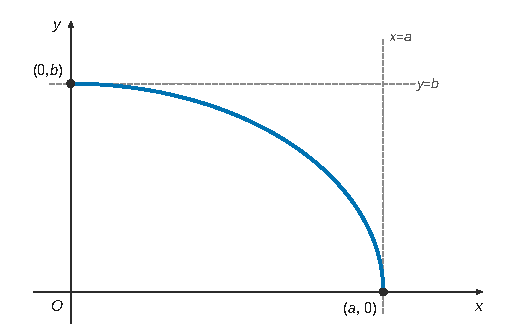
\includegraphics{figures/q7-courbe-cf.pdf}
\caption*{Figure 1 --- Tracé de 𝒞\_f (Q7) : tangente horizontale y = b en (0, b),
demi-tangente verticale x = a en (a, 0) ; tracé avec a = 3, b = 2}
\end{figure}

Tracé attendu : les deux tangentes tracées, points et axes nommés.

\begin{piege}

Faire arriver la courbe en \((a,0)\) avec une pente finie, comme un morceau de parabole : le tracé contredit alors Q6.

\end{piege}

\hypertarget{question-8}{%
\subsection{Question 8}\label{question-8}}

\begin{indication}{1}

Quelles symétries laissent invariante l'équation \(\frac{x^2}{a^2}+\frac{y^2}{b^2}=1\) ?

\end{indication}

\hypertarget{solution-7}{%
\subsubsection{Solution}\label{solution-7}}

L'équation est invariante par \((x,y)\mapsto(-x,y)\) et par \((x,y)\mapsto(x,-y)\). Donc \(\mathcal{E}\) est symétrique par rapport aux deux axes et à l'origine.
Un point de \(\mathcal{E}\) dans le premier quadrant vérifie \(x\in[0,a]\) et \(y=f(x)\). Donc \(\mathcal{E}\) est la réunion de \({\mathcal{C}}_f\) et de ses trois images par ces symétries.

\begin{figure}[H]
\centering
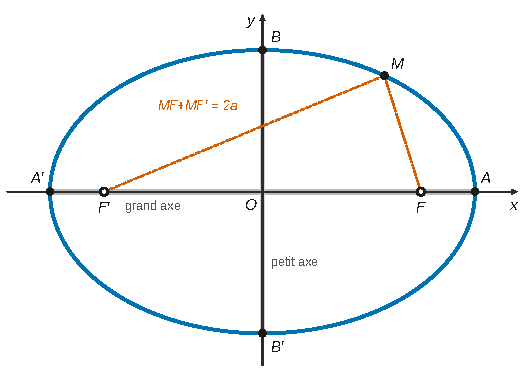
\includegraphics{figures/q8-ellipse-foyers.pdf}
\caption*{Figure 2 --- L'ellipse ℰ (Q8) : sommets A, A′, B, B′, foyers F, F′ sur
le grand axe, et un point M avec MF + MF′ = 2a ; tracé avec a = 3, b =
2, c = √5}
\end{figure}

Les tangentes sont verticales en \(A(a,0)\) et \(A'(-a,0)\). Elles sont horizontales en \(B(0,b)\) et \(B'(0,-b)\).
Comme \(b<a\), l'ellipse \(\mathcal{E}\) est allongée horizontalement. Ses foyers \(F(c,0)\) et \(F'(-c,0)\) sont strictement entre le centre et les sommets.

\begin{piege}

Placer les foyers sur le petit axe, ou à l'extérieur de l'ellipse. Ici \(0<c<a\).

\end{piege}

\hypertarget{iii-paramuxe8tres-de-lellipse}{%
\subsection{III --- Paramètres de l'ellipse}\label{iii-paramuxe8tres-de-lellipse}}

\hypertarget{question-9}{%
\subsection{Question 9}\label{question-9}}

\begin{indication}{1}

Divisez l'encadrement \(0<c<a\) par \(a\), puis réécrivez \(b\).

\end{indication}

\hypertarget{solution-8}{%
\subsubsection{Solution}\label{solution-8}}

Les inégalités \(0<c<a\) et \(a>0\) donnent \(\boxed{e\in\,]0,1[}\). Puis \(\boxed{c=ae}\).
En utilisant \(a>0\) pour sortir \(a\) de la racine :
\equationajustee{\boxed{\begin{aligned}
b&=\sqrt{a^2-a^2e^2}\\
&=a\sqrt{1-e^2}.
\end{aligned}}}

\hypertarget{question-10}{%
\subsection{Question 10}\label{question-10}}

\begin{indication}{1}

Raisonnez à \(a\) fixé et suivez \(b\) et \(c\) grâce aux formules de Q9.

\end{indication}

\hypertarget{solution-9}{%
\subsubsection{Solution}\label{solution-9}}

À \(a\) fixé, \(b=a\sqrt{1-e^2}\) et \(c=ae\).
- \textbf{Si \(e\) est proche de zéro}, alors \(b\approx a\) et \(c\approx0\). L'ellipse est presque le cercle de centre \(O\) et de rayon \(a\) ; les foyers sont presque au centre.
- \textbf{Si \(e\) est proche de 1}, alors \(b\approx0\) et \(c\approx a\). L'ellipse est très aplatie le long du grand axe \([A'A]\), et les foyers sont proches des sommets.

\begin{methode}

L'excentricité mesure la \textbf{forme}, pas la taille : deux ellipses de même \(e\) sont semblables. D'où l'intérêt de fixer \(a\) pour comparer. Pour les planètes, \(e\) est petit (orbites presque circulaires).

\end{methode}

\hypertarget{partie-b-uxe9tude-du-mouvement-des-planuxe8tes-massives-du-systuxe8me-solaire-sans-nuxe9gliger-les-interactions}{%
\section{Partie B --- Étude du mouvement des planètes massives du système solaire sans négliger les interactions}\label{partie-b-uxe9tude-du-mouvement-des-planuxe8tes-massives-du-systuxe8me-solaire-sans-nuxe9gliger-les-interactions}}

On transforme les relations de Lagrange-Laplace en un système \(H''=AH\), qu'on découple en diagonalisant \(A\). Outils : dérivation de vecteurs, critère de diagonalisabilité, équations \(y''+\omega^2y=0\).

\hypertarget{question-11}{%
\subsection{Question 11}\label{question-11}}

\begin{indication}{1}

\(G_t\) est la dérivée de \(H_t\). De même, \(K_t\) est celle de \(L_t\). Laquelle des deux relations faut-il dériver ?

\end{indication}

\begin{indication}{2}

Dérivez \(G_t=BL_t\) ligne par ligne, en utilisant que \(B\) est constante, puis injectez l'autre relation.

\end{indication}

\hypertarget{solution-10}{%
\subsubsection{Solution}\label{solution-10}}

Avec \(B=(\beta_{ij})\) constante, on a \(h_i'(t)=\sum_j\beta_{ij}l_j(t)\). Les \(l_j\) étant dérivables, on dérive :
\equationajustee{h_i''(t)=\sum_j\beta_{ij}l_j'(t),}
soit \(F_t=BK_t\). Avec \(K_t=-BH_t\) :
\equationajustee{\boxed{\begin{aligned}
F_t&=-B^2H_t\\
&=AH_t,\\
\text{avec}\quad A&=-B^2.
\end{aligned}}}

\begin{jury}

Une dérivation de produit matriciel \((BL_t)'=BL_t'\) doit être justifiée par la constance de \(B\) : l'énoncé insiste sur ce point, il faut s'en servir explicitement.

\end{jury}

\hypertarget{question-12}{%
\subsection{Question 12}\label{question-12}}

\begin{indication}{1}

Combien de valeurs propres distinctes \(A\) possède-t-elle, et dans quel corps ? Quel critère du cours s'applique ?

\end{indication}

\hypertarget{solution-11}{%
\subsubsection{Solution}\label{solution-11}}

La matrice \(A\in{\mathcal{M}}_3(\mathbb{R})\) a trois valeurs propres réelles deux à deux distinctes (\(\lambda_1<\lambda_2<\lambda_3\)) : elle est diagonalisable dans \({\mathcal{M}}_3(\mathbb{R})\).
Concrètement, des vecteurs propres associés \(X_1,X_2,X_3\) forment une famille libre, donc une base de \({\mathbb{R}}^3\).
La matrice \(Q\) de colonnes \(X_1,X_2,X_3\) est inversible. Elle vérifie \(AQ=Q\Delta\), avec \(\Delta=\mathrm{diag}(\lambda_1,\lambda_2,\lambda_3)\) :
\equationajustee{\boxed{A=Q\,\Delta\,Q^{-1},\quad Q\in{\mathrm{GL}}_3(\mathbb{R}).}}

\begin{piege}

Invoquer le théorème spectral : rien ne dit que \(A=-B^2\) soit symétrique.

\end{piege}

\hypertarget{question-13}{%
\subsection{Question 13}\label{question-13}}

\begin{indication}{1}

Dérivez deux fois \(Y_t=Q^{-1}H_t\) et utilisez successivement Q11 et Q12.

\end{indication}

\hypertarget{solution-12}{%
\subsubsection{Solution}\label{solution-12}}

La matrice \(Q^{-1}\) étant constante, \(Y\) est deux fois dérivable, et
\equationajustee{\begin{aligned}
Y_t''&=Q^{-1}H_t''\\
&=Q^{-1}AH_t\\
&=Q^{-1}Q\Delta Q^{-1}H_t\\
&=\Delta Y_t.
\end{aligned}}
Ligne par ligne, pour \(i\in\{1,2,3\}\) :
\equationajustee{\boxed{y_i''-\lambda_iy_i=0,}}
soit, avec \(\omega_i=\sqrt{-\lambda_i}>0\), \(y_i''+\omega_i^2y_i=0\).

\begin{methode}

Diagonaliser pour \textbf{découpler} : dans la base propre, le système \(H''=AH\) devient trois équations scalaires indépendantes. La même idée sert pour \(X'=AX\).

\end{methode}

\hypertarget{question-14}{%
\subsection{Question 14}\label{question-14}}

\begin{indication}{1}

Écrivez l'équation caractéristique ; le signe de \(\lambda_i\) décide de la nature des solutions.

\end{indication}

\hypertarget{solution-13}{%
\subsubsection{Solution}\label{solution-13}}

L'équation \(r^2=\lambda_i<0\) a pour racines \(\pm i\omega_i\). Donc
\equationajustee{\boxed{y_i(t)=\alpha_i\cos\big(\sqrt{-\lambda_i}\,t\big)+\beta_i\sin\big(\sqrt{-\lambda_i}\,t\big),\quad(\alpha_i,\beta_i)\in{\mathbb{R}}^2,}}
ou encore \(y_i(t)=C_i\cos(\omega_it-\varphi_i)\) : une oscillation de pulsation \(\sqrt{-\lambda_i}\).

\begin{methode}

L'hypothèse \(\lambda_i<0\) donne des solutions bornées (oscillations) ; avec \(\lambda_i>0\) on aurait des exponentielles \(e^{\pm\sqrt{\lambda_i}t}\). Le mouvement de chaque planète, \(h_k=\sum_jq_{kj}y_j\), superpose trois oscillations de périodes en général incommensurables.

\end{methode}

\hypertarget{question-15}{%
\subsection{Question 15}\label{question-15}}

\begin{indication}{1}

Pour l'inversibilité : \(A\) est inversible (pourquoi ?). Reliez \(\det A\) à \(\det B\). Ou bien comparez \(\ker B\) et \(\ker A\).

\end{indication}

\begin{indication}{2}

Pour les \(l_i\), renversez la relation qui donne \(L_t\) sans intégration.

\end{indication}

\hypertarget{solution-14}{%
\subsubsection{Solution}\label{solution-14}}

La matrice \(A\) est semblable à \(\Delta\), donc \(\det A=\lambda_1\lambda_2\lambda_3\neq0\). Or
\equationajustee{\begin{aligned}
\det A&=\det(-B^2)\\
&=(-1)^3(\det B)^2.
\end{aligned}}
Donc \(\det B\neq0\) :
\equationajustee{\boxed{B\in{\mathrm{GL}}_3(\mathbb{R}).}}
Autre voie : si \(BX=0\), alors \(AX=-B(BX)=0\), donc \(X=0\).

De \(Y_t=Q^{-1}H_t\) :
\equationajustee{\boxed{\begin{aligned}
H_t&=QY_t,\\
h_i&=\sum_{j=1}^3q_{ij}\,y_j.
\end{aligned}}}
De \(G_t=BL_t\), on tire
\equationajustee{\begin{aligned}
L_t&=B^{-1}G_t\\
&=B^{-1}H_t'\\
&=B^{-1}QY_t',
\end{aligned}}
d'où
\equationajustee{\boxed{\begin{aligned}
L_t&=B^{-1}Q\,Y_t',\\
l_i&=\sum_{j=1}^3r_{ij}\,y_j',
\end{aligned}}}
où \(B^{-1}Q=(r_{ij})\).

\begin{piege}

Partir de \(K_t=-BH_t\), soit \(L_t'=-BQY_t\), impose d'intégrer. Cela fait apparaître une constante qu'il faudrait ensuite identifier. La relation \(G_t=BL_t\) donne \(L_t\) directement.

Les deux voies concordent. Comme \(y_j''=\lambda_jy_j\), une primitive de \(Y\) est \(\Delta^{-1}Y'\).
Et \(-BQ\Delta^{-1}=-BA^{-1}Q=B^{-1}Q\), puisque \(A^{-1}=-B^{-2}\).

\end{piege}

\hypertarget{partie-c-muxe9thode-de-le-verrier-pour-duxe9terminer-les-valeurs-propres}{%
\section{Partie C --- Méthode de Le Verrier pour déterminer les valeurs propres}\label{partie-c-muxe9thode-de-le-verrier-pour-duxe9terminer-les-valeurs-propres}}

On montre que les coefficients du polynôme caractéristique d'une matrice carrée d'ordre 3 s'obtiennent à partir des seules traces de \(A\), \(A^2\), \(A^3\), puis on applique la méthode à un exemple.

\hypertarget{i-ruxe9solution-des-uxe9quations}{%
\subsection{I --- Résolution des équations}\label{i-ruxe9solution-des-uxe9quations}}

\hypertarget{question-16}{%
\subsection{Question 16}\label{question-16}}

\begin{indication}{1}

Écrivez le coefficient diagonal \((i,i)\) d'un produit, puis sommez.

\end{indication}

\begin{indication}{2}

Pour deux matrices semblables, groupez \(P^{-1}MP\) en un produit de deux facteurs bien choisis.

\end{indication}

\hypertarget{solution-15}{%
\subsubsection{Solution}\label{solution-15}}

Une somme finie ne dépend pas de l'ordre de sommation, donc
\equationajustee{\begin{aligned}
\mathrm{Tr}(AB)&=\sum_i\sum_ja_{ij}b_{ji}\\
&=\sum_j\sum_ib_{ji}a_{ij}\\
&=\mathrm{Tr}(BA).
\end{aligned}}
Si \(N=P^{-1}MP\), alors
\equationajustee{\begin{aligned}
\mathrm{Tr}(N)&=\mathrm{Tr}\big(P^{-1}(MP)\big)\\
&=\mathrm{Tr}\big((MP)P^{-1}\big)\\
&=\mathrm{Tr}(M).
\end{aligned}}
\textbf{Deux matrices semblables ont donc même trace.}

\begin{piege}

\(\mathrm{Tr}(ABC)=\mathrm{Tr}(BCA)\) (permutation circulaire), mais en général \(\mathrm{Tr}(ABC)\neq\mathrm{Tr}(ACB)\).

\end{piege}

\hypertarget{question-17}{%
\subsection{Question 17}\label{question-17}}

\begin{indication}{1}

Exprimez \(A^k\) à l'aide de \(\Delta^k\) : les \(Q^{-1}Q\) se simplifient.

\end{indication}

\hypertarget{solution-16}{%
\subsubsection{Solution}\label{solution-16}}

Par récurrence immédiate, \(A^k=Q\Delta^kQ^{-1}\), avec \(\Delta^k=\mathrm{diag}(\lambda_1^k,\lambda_2^k,\lambda_3^k)\). Par Q16 :
\equationajustee{\boxed{\begin{aligned}
\mathrm{Tr}(A)&=S_1,\\
\mathrm{Tr}(A^2)&=S_2,\\
\mathrm{Tr}(A^3)&=S_3.
\end{aligned}}}

\begin{piege}

En général, \(\mathrm{Tr}(A^2)\neq\mathrm{Tr}(A)^2\). C'est justement l'écart entre \(S_1^2\) et \(S_2\) qui donne \(\alpha_1\).

\end{piege}

\hypertarget{question-18}{%
\subsection{Question 18}\label{question-18}}

\begin{indication}{1}

Le polynôme caractéristique est invariant par similitude. Celui d'une matrice diagonale se lit directement.

\end{indication}

\hypertarget{solution-17}{%
\subsubsection{Solution}\label{solution-17}}

On a \(XI_3-A=Q(XI_3-\Delta)Q^{-1}\), d'où \(P_A=\det(XI_3-\Delta)\) :
\equationajustee{\boxed{P_A=(X-\lambda_1)(X-\lambda_2)(X-\lambda_3),}}
et, en développant et en identifiant (\(\alpha_3=1\)),
\equationajustee{\boxed{\begin{aligned}
\alpha_2&=-(\lambda_1+\lambda_2+\lambda_3),\\
\alpha_1&=\lambda_1\lambda_2+\lambda_1\lambda_3+\lambda_2\lambda_3,\\
\alpha_0&=-\lambda_1\lambda_2\lambda_3.
\end{aligned}}}

\begin{piege}

Avec la convention \(\det(A-XI_3)\), tous les coefficients changent de signe et Q21 donnerait \(-R\). Annoncez la convention \(\det(XI_3-A)\), qui est aussi la seule compatible avec la valeur admise de \(\alpha_0\).

\end{piege}

\hypertarget{question-19}{%
\subsection{Question 19}\label{question-19}}

\begin{indication}{1}

Développez \(S_1^2=(\lambda_1+\lambda_2+\lambda_3)^2\).

\end{indication}

\hypertarget{solution-18}{%
\subsubsection{Solution}\label{solution-18}}

On a \(\alpha_2=-S_1\), et
\equationajustee{\begin{aligned}
S_1^2&=S_2+2(\lambda_1\lambda_2+\lambda_1\lambda_3+\lambda_2\lambda_3)\\
&=S_2+2\alpha_1.
\end{aligned}}
Donc
\equationajustee{\boxed{\begin{aligned}
\alpha_2&=-S_1,\\
\alpha_1&=\frac{S_1^2-S_2}{2}.
\end{aligned}}}
Avec Q17 et la valeur admise de \(\alpha_0\), le polynôme \(P_A\) ne dépend que des traces des trois premières puissances de \(A\).

\begin{methode}

Test de contrôle en trente secondes : prendre \(A=I_3\), pour laquelle \(S_1=S_2=S_3=3\). On trouve \(\alpha_2=-3\), \(\alpha_1=3\) et \(\alpha_0=-1\). C'est bien \((X-1)^3\).

\end{methode}

\hypertarget{ii-uxe9tude-dun-cas-particulier}{%
\subsection{II --- Étude d'un cas particulier}\label{ii-uxe9tude-dun-cas-particulier}}

On pose \(N=2A\), ce qui évite les fractions : \(A^k=N^k/2^k\), avec
\equationajustee{N=\begin{pmatrix}-4&11&13\\0&1&7\\0&7&1\end{pmatrix}.}

\hypertarget{question-20}{%
\subsection{Question 20}\label{question-20}}

\begin{indication}{1}

Sur \(\mathbb{C}\), que peut-on dire de tout polynôme non constant ? Quel critère de trigonalisation s'applique alors ?

\end{indication}

\begin{indication}{2}

Pour le second volet, repérez ce que Q17 et Q18 utilisaient vraiment de la forme diagonale, et vérifiez que cela reste vrai pour une matrice triangulaire.

\end{indication}

\hypertarget{solution-19}{%
\subsubsection{Solution}\label{solution-19}}

Le polynôme \(P_A\) est scindé sur \(\mathbb{C}\) (théorème de d'Alembert-Gauss), donc \(A\) est trigonalisable sur ce corps :
\equationajustee{\boxed{A=QTQ^{-1},}}
avec \(T\) triangulaire supérieure et \(Q\in{\mathrm{GL}}_3(\mathbb{C})\).

Soient \(\mu_1,\mu_2,\mu_3\) les coefficients diagonaux de \(T\). Les puissances \(T^k\) sont triangulaires supérieures, de diagonale \((\mu_i^k)\).
Comme Q16 vaut sur \(\mathbb{C}\), on en déduit
\equationajustee{\mathrm{Tr}(A^k)=\sum_i\mu_i^k.}
De plus,
\equationajustee{\begin{aligned}
P_A&=\det(XI_3-T)\\
&=\prod_i(X-\mu_i).
\end{aligned}}
Les calculs de Q17--Q19 se répètent à l'identique : \textbf{oui, les relations de Q19 restent valables}, avec \(S_k=\mathrm{Tr}(A^k)\) et les valeurs propres complexes comptées avec multiplicité.

\begin{methode}

Pour la trace des puissances et le polynôme caractéristique, une forme triangulaire suffit : seule la diagonale compte. Les \(S_k\), traces de matrices réelles, restent réels.

\end{methode}

\hypertarget{question-21}{%
\subsection{Question 21}\label{question-21}}

\begin{indication}{1}

Calculez \(N^2\) puis \(N^3=N^2N\) ; la structure triangulaire par blocs simplifie les calculs.

\end{indication}

\begin{indication}{2}

Appliquez ensuite Q19, légitimée par Q20.

\end{indication}

\hypertarget{solution-20}{%
\subsubsection{Solution}\label{solution-20}}

\equationajustee{\begin{aligned}
N^2&=\begin{pmatrix}16&58&38\\0&50&14\\0&14&50\end{pmatrix},\\
N^3&=\begin{pmatrix}-64&500&652\\0&148&364\\0&364&148\end{pmatrix}.
\end{aligned}}
On a donc \(\mathrm{Tr}(N)=-2\), \(\mathrm{Tr}(N^2)=116\) et \(\mathrm{Tr}(N^3)=232\). En divisant respectivement par 2, 4 et 8 :
\equationajustee{\boxed{\begin{aligned}
\mathrm{Tr}(A)&=-1,\\
\mathrm{Tr}(A^2)&=29,\\
\mathrm{Tr}(A^3)&=29.
\end{aligned}}}
Alors
\equationajustee{\begin{aligned}
\alpha_2&=1,\\
\alpha_1&=\frac{1-29}{2}\\
&=-14,\\
\alpha_0&=\frac{-87+1-58}{6}\\
&=-24.
\end{aligned}}
Donc
\equationajustee{\boxed{\begin{aligned}
P_A&=X^3+X^2-14X-24\\
&=R.
\end{aligned}}}

\begin{methode}

Recoupement : \(N\) est triangulaire par blocs, de la forme \(\begin{pmatrix}-4&*\\0&S\end{pmatrix}\). Le bloc \(S=\begin{pmatrix}1&7\\7&1\end{pmatrix}\) a pour valeurs propres \(8\) et \(-6\).
Donc \(\mathrm{Tr}(N^k)=(-4)^k+8^k+(-6)^k\), ce qui redonne bien −2, 116 et 232 pour k = 1, 2, 3.

\end{methode}

\hypertarget{question-22}{%
\subsection{Question 22}\label{question-22}}

\begin{indication}{1}

Cherchez une racine entière parmi les diviseurs de \(24\).

\end{indication}

\hypertarget{solution-21}{%
\subsubsection{Solution}\label{solution-21}}

On a \(R(-2)=0\), d'où la factorisation
\equationajustee{\begin{aligned}
R&=(X+2)(X^2-X-12)\\
&=(X+2)(X+3)(X-4).
\end{aligned}}
Donc
\equationajustee{\boxed{\mathrm{Sp}(A)=\{-3,-2,4\}.}}
Trois valeurs propres distinctes : \(A\) est diagonalisable dans \({\mathcal{M}}_3(\mathbb{R})\).

\hypertarget{question-23}{%
\subsection{Question 23}\label{question-23}}

\begin{indication}{1}

Résolvez \((N-2\lambda I_3)X=0\) pour chacune des trois valeurs propres.

\end{indication}

\begin{indication}{2}

Pour \(\lambda=-2\), la première colonne de \(N+4I_3\) est nulle.

\end{indication}

\hypertarget{solution-22}{%
\subsubsection{Solution}\label{solution-22}}

\emph{Pour \(\lambda=-2\).} Le système
\equationajustee{\begin{aligned}
11y+13z&=0,\\
5y+7z&=0,\\
7y+5z&=0
\end{aligned}}
impose \(y=z=0\), car \(25-49\neq0\) : \(X_1=(1,0,0)^\top\).

\emph{Pour \(\lambda=-3\).} Les équations sont
\equationajustee{\begin{aligned}
2x+11y+13z&=0,\\
y+z&=0.
\end{aligned}}
Elles donnent \(y=-z\), puis \(x=-z\) : \(X_2=(1,1,-1)^\top\).

\emph{Pour \(\lambda=4\).} Les équations sont
\equationajustee{\begin{aligned}
-12x+11y+13z&=0,\\
y&=z.
\end{aligned}}
Elles donnent \(x=2z\) : \(X_3=(2,1,1)^\top\).

Vérification : \(NX_1=-4X_1\), \(NX_2=-6X_2\), \(NX_3=8X_3\). Donc
\equationajustee{\boxed{\begin{aligned}
Q&=\begin{pmatrix}1&1&2\\0&1&1\\0&-1&1\end{pmatrix},\\
Q^{-1}AQ&=\mathrm{diag}(-2,-3,4),\\
\det Q&=2.
\end{aligned}}}

\begin{piege}

L'ordre des valeurs propres sur la diagonale est celui des colonnes de \(Q\). Et c'est \(Q^{-1}AQ\) qui est diagonale : les vecteurs propres sont \textbf{en colonnes}.

\end{piege}

\hypertarget{partie-d-perturbation-sur-une-matrice-dordre-3}{%
\section{Partie D --- Perturbation sur une matrice d'ordre 3}\label{partie-d-perturbation-sur-une-matrice-dordre-3}}

On caractérise le spectre de \(D(t)=D+tUU^\top\) par l'équation scalaire \(F(\lambda)=\frac1t\), puis on suit ses valeurs propres comme fonctions de \(t\).
Outils : calcul matriciel, théorème de la bijection, limites, taux d'accroissement. Notation :
\equationajustee{F(\lambda)=\frac{u^2}{\lambda-a}+\frac{v^2}{\lambda-b}+\frac{w^2}{\lambda-c},}
et \(u^2,v^2,w^2>0\).

\hypertarget{i-solutions-et-spectre}{%
\subsection{I --- Solutions et spectre}\label{i-solutions-et-spectre}}

\hypertarget{question-24}{%
\subsection{Question 24}\label{question-24}}

\begin{indication}{1}

\(\lambda I_3-D\) est diagonale : son inversibilité se lit sur la diagonale.

\end{indication}

\begin{indication}{2}

Partez de \(D(t)X=\lambda X\) et isolez le terme \(tU(U^\top X)\). Multipliez ensuite à gauche par \((\lambda I_3-D)^{-1}\), puis par \(U^\top\).

\end{indication}

\hypertarget{solution-23}{%
\subsubsection{Solution}\label{solution-23}}

La matrice \(\lambda I_3-D=\mathrm{diag}(\lambda-a,\lambda-b,\lambda-c)\) a ses coefficients diagonaux non nuls :
\equationajustee{\boxed{\lambda I_3-D\in{\mathrm{GL}}_3(\mathbb{R}).}}
Soit \(X\neq0\) tel que \(D(t)X=\lambda X\). Alors
\equationajustee{\begin{aligned}
(\lambda I_3-D)X&=tU(U^\top X),\\
X&=t(\lambda I_3-D)^{-1}U(U^\top X),
\end{aligned}}
puis
\equationajustee{\boxed{U^\top X=t\,U^\top(\lambda I_3-D)^{-1}UU^\top X.}}

\begin{piege}

Le produit \(U^\top X\) est un scalaire (matrice \(1\times1\)). En revanche, \(UU^\top=T\) est une matrice \(3\times3\) de rang 1. Les confondre rend la partie incompréhensible.

\end{piege}

\hypertarget{question-25}{%
\subsection{Question 25}\label{question-25}}

\begin{indication}{1}

La relation de Q24 est de la forme \(s=\kappa s\) avec \(s\) scalaire. Que faut-il exclure pour simplifier ?

\end{indication}

\begin{indication}{2}

Si \(s=U^\top X\) était nul, que deviendrait l'expression de \(X\) obtenue en Q24 ?

\end{indication}

\hypertarget{solution-24}{%
\subsubsection{Solution}\label{solution-24}}

Soit \(s=U^\top X\). Si \(s=0\), alors \(X=t(\lambda I_3-D)^{-1}U\,s=0\), ce qui est exclu pour un vecteur propre.
Donc \(s\neq0\), et l'on simplifie : \(t\,U^\top(\lambda I_3-D)^{-1}U=1\). Comme \(t\neq0\),
\equationajustee{\boxed{U^\top(\lambda I_3-D)^{-1}U=\frac1t.}}

\begin{jury}

Toute simplification par une quantité doit être précédée de la preuve que cette quantité est non nulle : c'est l'unique difficulté de la question.

\end{jury}

\hypertarget{question-26}{%
\subsection{Question 26}\label{question-26}}

\begin{indication}{1}

Explicitez le produit avec l'inverse diagonal de Q24.

\end{indication}

\hypertarget{solution-25}{%
\subsubsection{Solution}\label{solution-25}}

On a
\equationajustee{(\lambda I_3-D)^{-1}U=\Big(\frac u{\lambda-a},\frac v{\lambda-b},\frac w{\lambda-c}\Big)^\top,}
donc \(U^\top(\lambda I_3-D)^{-1}U=F(\lambda)\).
Q25 donne alors \(\boxed{F(\lambda)=\frac1t}\) : \(\lambda\) est solution de \((E_t)\).

\hypertarget{question-27}{%
\subsection{Question 27}\label{question-27}}

\begin{indication}{1}

\(F\) est définie sur une réunion de quatre intervalles. Calculez \(F'\) et son signe.

\end{indication}

\begin{indication}{2}

En chaque point singulier, un seul terme explose ; les deux autres restent bornés. Concluez sur chaque intervalle avec le théorème de la bijection.

\end{indication}

\hypertarget{solution-26}{%
\subsubsection{Solution}\label{solution-26}}

On note
\equationajustee{\begin{aligned}
I_1&=\,]-\infty,a[,\\
I_2&=\,]a,b[,\\
I_3&=\,]b,c[,\\
I_4&=\,]c,+\infty[.
\end{aligned}}
Sur chacun de ces intervalles,
\equationajustee{F'(\lambda)=-\frac{u^2}{(\lambda-a)^2}-\frac{v^2}{(\lambda-b)^2}-\frac{w^2}{(\lambda-c)^2}<0,}
donc \(F\) est strictement décroissante sur \textbf{chacun} des quatre intervalles. Limites :
\equationajustee{\begin{aligned}
\lim_{-\infty}F&=0^-,\\
\lim_{a^-}F&=-\infty,\\
\lim_{a^+}F&=+\infty,\\
\lim_{b^-}F&=-\infty,\\
\lim_{b^+}F&=+\infty,\\
\lim_{c^-}F&=-\infty,\\
\lim_{c^+}F&=+\infty,\\
\lim_{+\infty}F&=0^+.
\end{aligned}}
De plus, \(F\) est négative sur \(I_1\) et positive sur \(I_4\).

\begin{longtable}[]{@{}
  >{\raggedright\arraybackslash}p{(\columnwidth - 18\tabcolsep) * \real{0.1165}}
  >{\raggedright\arraybackslash}p{(\columnwidth - 18\tabcolsep) * \real{0.0930}}
  >{\raggedright\arraybackslash}p{(\columnwidth - 18\tabcolsep) * \real{0.1361}}
  >{\raggedright\arraybackslash}p{(\columnwidth - 18\tabcolsep) * \real{0.0609}}
  >{\raggedright\arraybackslash}p{(\columnwidth - 18\tabcolsep) * \real{0.1111}}
  >{\raggedright\arraybackslash}p{(\columnwidth - 18\tabcolsep) * \real{0.0609}}
  >{\raggedright\arraybackslash}p{(\columnwidth - 18\tabcolsep) * \real{0.1111}}
  >{\raggedright\arraybackslash}p{(\columnwidth - 18\tabcolsep) * \real{0.0609}}
  >{\raggedright\arraybackslash}p{(\columnwidth - 18\tabcolsep) * \real{0.1267}}
  >{\raggedright\arraybackslash}p{(\columnwidth - 18\tabcolsep) * \real{0.0930}}@{}}
\toprule\noalign{}
\begin{minipage}[b]{\linewidth}\raggedright
\(\lambda\)
\end{minipage} & \begin{minipage}[b]{\linewidth}\raggedright
\(-\infty\)
\end{minipage} & \begin{minipage}[b]{\linewidth}\raggedright
\end{minipage} & \begin{minipage}[b]{\linewidth}\raggedright
\(a\)
\end{minipage} & \begin{minipage}[b]{\linewidth}\raggedright
\end{minipage} & \begin{minipage}[b]{\linewidth}\raggedright
\(b\)
\end{minipage} & \begin{minipage}[b]{\linewidth}\raggedright
\end{minipage} & \begin{minipage}[b]{\linewidth}\raggedright
\(c\)
\end{minipage} & \begin{minipage}[b]{\linewidth}\raggedright
\end{minipage} & \begin{minipage}[b]{\linewidth}\raggedright
\(+\infty\)
\end{minipage} \\
\midrule\noalign{}
\endhead
\bottomrule\noalign{}
\endlastfoot
\(F'(\lambda)\) & & \(-\) & ‖ & \(-\) & ‖ & \(-\) & ‖ & \(-\) & \\
\(F\) & 0⁻ & décroît vers −∞ & ‖ & de +∞ à −∞ & ‖ & de +∞ à −∞ & ‖ & décroît de +∞ & 0⁺ \\
\end{longtable}

\(F\) réalise donc des bijections
\equationajustee{\begin{aligned}
I_1&\to\,]-\infty,0[,\\
I_2&\to\mathbb{R},\\
I_3&\to\mathbb{R},\\
I_4&\to\,]0,+\infty[,
\end{aligned}}
et
\equationajustee{\boxed{F\text{ s'annule exactement en }\rho_1\in\,]a,b[\text{ et }\rho_2\in\,]b,c[.}}

\begin{piege}

Écrire « \(F\) est décroissante sur \(\mathbb{R}\setminus\{a,b,c\}\) » : cet ensemble n'est pas un intervalle et le théorème de la bijection ne s'y applique pas.

\end{piege}

\begin{methode}

L'hypothèse \(u,v,w\neq0\) est essentielle. Si par exemple \(v=0\), alors \(b\) n'est plus une singularité de \(F\), qui n'a plus qu'un zéro.
De plus, \(b\) devient valeur propre de \(D(t)\), de vecteur propre \(e_2\). Le lien entre \((E_t)\) et le spectre se rompt.

\end{methode}

\hypertarget{question-28}{%
\subsection{Question 28}\label{question-28}}

\begin{indication}{1}

Coupez le graphe de \(F\) par la droite horizontale d'ordonnée \(\frac1t\). Le signe de \(\frac1t\) décide des branches concernées.

\end{indication}

\begin{indication}{2}

Pour placer une solution par rapport à \(\rho_i\), comparez \(\frac1t\) à \(0=F(\rho_i)\) et utilisez la décroissance.

\end{indication}

\hypertarget{solution-27}{%
\subsubsection{Solution}\label{solution-27}}

\begin{figure}[H]
\centering
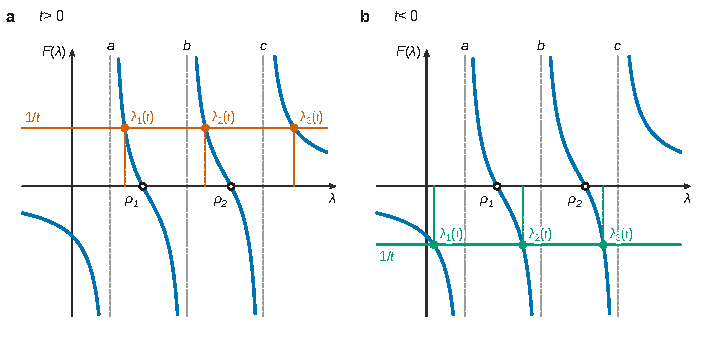
\includegraphics{figures/q28-graphe-f-droite-1-sur-t.pdf}
\caption*{Figure 3 --- Résolution graphique de (Eₜ) (Q28) : la droite d'ordonnée
1/t coupe le graphe de F en λ₁(t) \textless{} λ₂(t) \textless{} λ₃(t),
(a) pour t \textgreater{} 0, (b) pour t \textless{} 0 ; tracé avec a =
1, b = 3, c = 5, u² = v² = w² = 1}
\end{figure}

\emph{Cas \(t>0\).} Il n'y a pas de solution sur \(I_1\).
Il y en a une sur \(I_2\), inférieure à \(\rho_1\) car \(F(\lambda)=\frac1t>0=F(\rho_1)\).
Il y en a une sur \(I_3\), inférieure à \(\rho_2\), et une sur \(I_4\) :
\equationajustee{\boxed{a<\lambda_1(t)<\rho_1<b<\lambda_2(t)<\rho_2<c<\lambda_3(t).}}
\emph{Cas \(t<0\).} Il y a une solution sur \(I_1\).
Il y en a une sur \(I_2\), supérieure à \(\rho_1\).
Il y en a une sur \(I_3\), supérieure à \(\rho_2\), et aucune sur \(I_4\) :
\equationajustee{\boxed{\lambda_1(t)<a<\rho_1<\lambda_2(t)<b<\rho_2<\lambda_3(t)<c.}}
Dans les deux cas : exactement trois solutions, distinctes.

\begin{piege}

\(\lambda_1(t)\) est la plus petite solution. Elle n'est pas sur la même branche selon le signe de \(t\). Pour \(t>0\), elle est dans \(I_2\). Pour \(t<0\), elle est dans \(I_1\).

\end{piege}

\hypertarget{question-29}{%
\subsection{Question 29}\label{question-29}}

\begin{indication}{1}

Une inclusion vient de Q24--Q26, mais sous l'hypothèse \(\lambda\notin\{a,b,c\}\). Montrez d'abord que \(a,b,c\) ne sont pas valeurs propres de \(D(t)\).

\end{indication}

\begin{indication}{2}

Pour l'autre inclusion, la formule de \(X\) dans Q24 suggère un candidat vecteur propre fabriqué à partir de \(U\).

\end{indication}

\hypertarget{solution-28}{%
\subsubsection{Solution}\label{solution-28}}

Notons \(\mathcal{S}\) l'ensemble des solutions de \((E_t)\).

\emph{\(a\notin\mathrm{Sp}(D(t))\).} Supposons \(D(t)X=aX\). Alors
\equationajustee{\mathrm{diag}(0,a-b,a-c)\,X=tU(U^\top X).}
La première ligne donne \(tu(U^\top X)=0\), donc \(U^\top X=0\).
Alors \(x_2=x_3=0\), puis \(U^\top X=ux_1=0\) donne \(x_1=0\). Même argument pour \(b\) et \(c\).

\emph{\(\mathrm{Sp}(D(t))\subset\mathcal{S}\)} : par ce qui précède et Q24--Q26.

\emph{\(\mathcal{S}\subset\mathrm{Sp}(D(t))\).} Soit \(\lambda\) une solution. Le vecteur \(X=(\lambda I_3-D)^{-1}U\) est non nul, car sa première composante \(\frac u{\lambda-a}\) ne l'est pas.
On a \(DX=\lambda X-U\) et \(U^\top X=F(\lambda)=\frac1t\), donc
\equationajustee{\begin{aligned}
D(t)X&=\lambda X-U+tU\cdot\frac1t\\
&=\lambda X.
\end{aligned}}
Ainsi
\equationajustee{\boxed{\begin{aligned}
\mathcal{S}&=\mathrm{Sp}\big(D(t)\big)\\
&=\{\lambda_1(t),\lambda_2(t),\lambda_3(t)\}.
\end{aligned}}}

\begin{methode}

Pour montrer l'égalité d'un ensemble de solutions et d'un spectre : double inclusion, et pour le sens « solution \(\Rightarrow\) valeur propre », \textbf{exhiber} un vecteur propre. Le théorème spectral (\(D(t)\) symétrique réelle) ne dispense d'aucune des deux étapes.

\end{methode}

\hypertarget{ii-les-limites}{%
\subsection{II --- Les limites}\label{ii-les-limites}}

\hypertarget{question-30}{%
\subsection{Question 30}\label{question-30}}

\begin{indication}{1}

Existence des \(g_i\) : théorème de la bijection, déjà utilisé en Q27.

\end{indication}

\begin{indication}{2}

Pour les limites de \(g_2\), utilisez la monotonie (limite monotone), puis un raisonnement par l'absurde avec la continuité de \(F\).

\end{indication}

\hypertarget{solution-29}{%
\subsubsection{Solution}\label{solution-29}}

Chaque restriction \(F_{|I_i}\) est continue et strictement décroissante sur un intervalle, donc bijective sur \(F(I_i)\), de réciproque \(g_i\) continue strictement décroissante :
\equationajustee{\begin{aligned}
g_1&:\,]-\infty,0[\,\to I_1,\\
g_2&:\mathbb{R}\to I_2,\\
g_3&:\mathbb{R}\to I_3,\\
g_4&:\,]0,+\infty[\,\to I_4.
\end{aligned}}
Comme \(F(\rho_1)=0\) avec \(\rho_1\in I_2\), on a \(\boxed{g_2(0)=\rho_1}\).

La fonction \(g_2\) est décroissante et minorée par \(a\). Elle admet donc en \(+\infty\) une limite \(\ell\in[a,b[\).
Si \(\ell>a\), on aurait
\equationajustee{y=F\big(g_2(y)\big)\xrightarrow[y\to+\infty]{}F(\ell),}
limite finie : c'est absurde. De même en \(-\infty\). Donc
\equationajustee{\boxed{\begin{aligned}
\lim_{+\infty}g_2&=a,\\
\lim_{-\infty}g_2&=b.
\end{aligned}}}

\begin{piege}

La fonction \(g_2\) est décroissante. Sa limite en \(+\infty\) est donc la borne \textbf{inférieure} \(a\), pas \(b\).
Et \(g_2\) est définie sur \(\mathbb{R}\), à valeurs dans \(]a,b[\), et non l'inverse.

\end{piege}

\hypertarget{question-31}{%
\subsection{Question 31}\label{question-31}}

\begin{indication}{1}

Appariez les branches de Q28 et les réciproques de Q30, en n'oubliant pas que l'argument est \(\frac1t\).

\end{indication}

\hypertarget{solution-30}{%
\subsubsection{Solution}\label{solution-30}}

\equationajustee{\boxed{\begin{aligned}
\text{pour } t>0:\quad\lambda_1(t)&=g_2\Big(\frac1t\Big),\\
\lambda_2(t)&=g_3\Big(\frac1t\Big),\\
\lambda_3(t)&=g_4\Big(\frac1t\Big);
\end{aligned}}}
\equationajustee{\boxed{\begin{aligned}
\text{pour } t<0:\quad\lambda_1(t)&=g_1\Big(\frac1t\Big),\\
\lambda_2(t)&=g_2\Big(\frac1t\Big),\\
\lambda_3(t)&=g_3\Big(\frac1t\Big).
\end{aligned}}}
Les domaines sont respectés : \(\frac1t>0\) dans l'expression par \(g_4\). De même, \(\frac1t<0\) dans l'expression par \(g_1\).

\hypertarget{question-32}{%
\subsection{Question 32}\label{question-32}}

\begin{indication}{1}

Continuité sur \({\mathbb{R}}^*\) par composition ; il reste à comparer les limites en \(0^+\) et \(0^-\).

\end{indication}

\begin{indication}{2}

En \(0^-\), c'est la limite de \(g_1\) en \(-\infty\) qu'il faut : même argument qu'en Q30.

\end{indication}

\hypertarget{solution-31}{%
\subsubsection{Solution}\label{solution-31}}

Par Q31,
\equationajustee{\begin{aligned}
\lambda_1(t)&=g_2\Big(\frac1t\Big)\quad\text{pour } t>0,\\
\lambda_1(t)&=g_1\Big(\frac1t\Big)\quad\text{pour } t<0.
\end{aligned}}
Par composition, \(\lambda_1\) est continue sur \({\mathbb{R}}^*\).

En \(0^+\) : \(\frac1t\to+\infty\), donc \(\lambda_1(t)\to a\) par Q30.

En \(0^-\) : \(\frac1t\to-\infty\). La fonction \(g_1\) est décroissante et majorée par \(a\).
Elle admet donc en \(-\infty\) une limite finie \(\ell\leqslant a\). Si \(\ell<a\), on aurait \(y=F(g_1(y))\to F(\ell)\), fini : c'est absurde.
Donc \(\lambda_1(t)\to a\). En posant \(\boxed{\lambda_1(0)=a}\), \(\lambda_1\) est continue sur \(\mathbb{R}\).

\begin{piege}

Les deux côtés passent par des réciproques \textbf{différentes} (\(g_2\) et \(g_1\)) : traiter un seul côté ne suffit pas.

\end{piege}

\hypertarget{question-33}{%
\subsection{Question 33}\label{question-33}}

\begin{indication}{1}

Sur \({\mathbb{R}}^*\) : dérivée d'une bijection réciproque (\(F'\) ne s'annule pas). En \(0\) : revenez au taux d'accroissement.

\end{indication}

\begin{indication}{2}

Posez \(\varepsilon(t)=\lambda_1(t)-a\) et écrivez \(F(\lambda_1(t))=\frac1t\). Multipliez par \(t\) : quels termes tendent vers \(0\) ?

\end{indication}

\hypertarget{solution-32}{%
\subsubsection{Solution}\label{solution-32}}

Les fonctions \(g_1\) et \(g_2\) sont dérivables, car \(F'\) ne s'annule pas. Donc \(\lambda_1\) est dérivable sur \({\mathbb{R}}^*\) par composition.

\emph{En \(0\).} On a \(\varepsilon(t)\neq0\) pour \(t\neq0\) (Q28). De plus, \(\varepsilon(t)\to0\) (Q32).
En multipliant \(F(\lambda_1(t))=\frac1t\) par \(t\) :
\equationajustee{\frac{tu^2}{\varepsilon(t)}+t\Big(\frac{v^2}{\lambda_1(t)-b}+\frac{w^2}{\lambda_1(t)-c}\Big)=1.}
La parenthèse tend vers la limite finie \(\frac{v^2}{a-b}+\frac{w^2}{a-c}\). Donc \(\frac{tu^2}{\varepsilon(t)}\to1\), et
\equationajustee{\begin{aligned}
\frac{\lambda_1(t)-\lambda_1(0)}{t}&=\frac{\varepsilon(t)}t\\
&\xrightarrow[t\to0]{}u^2.
\end{aligned}}
Ainsi \(\lambda_1\) est dérivable sur \(\mathbb{R}\), et
\equationajustee{\boxed{\begin{aligned}
\lambda_1'(0)&=u^2,\\
\lambda_2'(0)&=v^2,\\
\lambda_3'(0)&=w^2.
\end{aligned}}}

\begin{methode}

Contrôle par la trace : \(\lambda_1+\lambda_2+\lambda_3=\mathrm{Tr}\,D(t)=a+b+c+t(u^2+v^2+w^2)\), dont la dérivée vaut bien \(u^2+v^2+w^2\). Résultat cohérent avec la diagonale \((a+tu^2,b+tv^2,c+tw^2)\) de \(D(t)\).

\end{methode}

\hypertarget{question-34}{%
\subsection{Question 34}\label{question-34}}

\begin{indication}{1}

En \(\pm\infty\), on a \(\frac1t\to0\). Utilisez Q31, et le comportement de \(g_2\) en zéro et de \(g_1\) à gauche de zéro.

\end{indication}

\begin{indication}{2}

Pour \(g_1\) en \(0^-\), raisonnez comme en Q30. Une limite finie contredirait \(F(g_1(y))=y\to0\), puisque \(F<0\) sur \(I_1\). Pour le commentaire, rassemblez Q28, Q32 et Q33.

\end{indication}

\hypertarget{solution-33}{%
\subsubsection{Solution}\label{solution-33}}

Pour \(t>0\), \(\lambda_1(t)=g_2(\frac1t)\). Quand \(t\to+\infty\), la continuité de \(g_2\) donne \(\lambda_1(t)\to g_2(0)=\rho_1\).

Pour \(t<0\), \(\lambda_1(t)=g_1(\frac1t)\). Quand \(t\to-\infty\), on a \(\frac1t\to0^-\).
La fonction \(g_1\) est décroissante. Si elle était minorée près de \(0^-\), elle aurait une limite finie \(m<a\).
On aurait alors \(y=F(g_1(y))\to F(m)<0\), alors que \(y\to0\) : c'est absurde. Donc \(g_1(y)\to-\infty\), et
\equationajustee{\boxed{\begin{aligned}
\lim_{t\to+\infty}\lambda_1(t)&=\rho_1,\\
\lim_{t\to-\infty}\lambda_1(t)&=-\infty.
\end{aligned}}}

\begin{figure}[H]
\centering
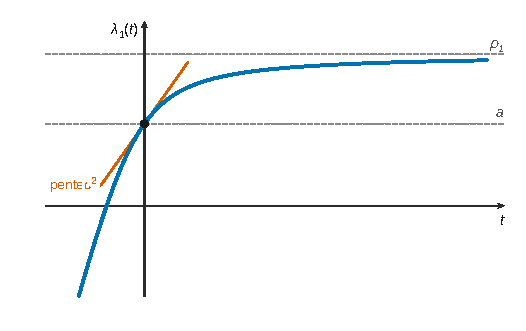
\includegraphics{figures/q34-allure-lambda1.pdf}
\caption*{Figure 4 --- Allure de λ₁ prolongée (Q32--Q34) : égale à a en 0 avec la
pente u², tendant vers ρ₁ en +∞ et vers −∞ en −∞ ; courbe calculée avec
a = 1, b = 3, c = 5, u² = v² = w² = 1}
\end{figure}

Commentaires sur les spectres de \(D\) et de \(D(t)\).

\textbf{Continuité.} Chaque \(\lambda_i(t)\) tend vers la valeur propre correspondante de \(D\) quand \(t\to0\). Une petite erreur sur la matrice ne déplace que peu le spectre.

\textbf{Sensibilité au premier ordre.}
\equationajustee{\begin{aligned}
\lambda_1(t)&=a+u^2t+o(t),\\
\lambda_2(t)&=b+v^2t+o(t),\\
\lambda_3(t)&=c+w^2t+o(t).
\end{aligned}}

\textbf{Entrelacement.} Pour \(t>0\) :
\equationajustee{a<\lambda_1(t)<b<\lambda_2(t)<c<\lambda_3(t).}
Pour \(t<0\) :
\equationajustee{\lambda_1(t)<a<\lambda_2(t)<b<\lambda_3(t)<c.}

\textbf{Grande perturbation.} Quand \(t\to+\infty\), \(\lambda_1\to\rho_1\) et \(\lambda_2\to\rho_2\) restent bornées. Seule \(\lambda_3\) tend alors vers \(+\infty\).
Quand \(t\to-\infty\), \(\lambda_2\to\rho_1\) et \(\lambda_3\to\rho_2\). Seule \(\lambda_1\) tend alors vers \(-\infty\).
Une perturbation de rang 1 n'envoie à l'infini qu'une seule valeur propre.

\begin{piege}

Croire par symétrie que \(\lambda_1\to\rho_1\) aussi en \(-\infty\) : les deux limites sont de natures différentes (finie d'un côté, infinie de l'autre).

\end{piege}

\begin{methode}

Un commentaire demandé se nourrit des résultats établis : citez les questions (continuité Q32, dérivée Q33, encadrements Q28) plutôt que des généralités.

\end{methode}

\hypertarget{bilan}{%
\section{Bilan}\label{bilan}}

\textbf{Méthodes à retenir.}
- Majorer une différence de distances par l'inégalité triangulaire appliquée deux fois ; regrouper des facteurs conjugués pour éliminer les racines carrées.
- Tangente verticale : limite infinie du taux d'accroissement, équation \(x=x_0\).
- Diagonaliser pour découpler un système différentiel linéaire à coefficients constants ; résoudre \(y''+\omega^2y=0\).
- \(\mathrm{Tr}(AB)=\mathrm{Tr}(BA)\), invariance de la trace et du polynôme caractéristique par similitude ; lien entre coefficients du polynôme caractéristique et sommes de Newton (relations coefficients-racines).
- Trigonaliser sur \(\mathbb{C}\) pour étendre un résultat démontré dans le cas diagonalisable.
- Étudier une équation \(F(\lambda)=k\) branche par branche avec le théorème de la bijection ; limites des réciproques par monotonie et contradiction.
- Dériver en un point délicat par le taux d'accroissement, en exploitant une relation implicite.

\textbf{Prérequis à revoir.} Critère de diagonalisabilité (valeurs propres distinctes), trigonalisation, convention \(\det(XI_n-A)\), théorème de la bijection et dérivée d'une réciproque, limite monotone.

\textbf{Questions transposables.} L'équation réduite de l'ellipse (Q1--Q5) ; la méthode de Le Verrier et le polynôme caractéristique par les traces (Q16--Q21), qui se généralise aux identités de Newton ; la perturbation de rang 1 \(D+tUU^\top\) et l'entrelacement des valeurs propres (Q24--Q34), classique aussi bien en algèbre linéaire qu'en analyse numérique.

\end{document}
